\documentclass[11pt]{article}
\usepackage{caption}
\usepackage{anysize}
\usepackage{fancyhdr}
\usepackage{graphicx}
\usepackage{subcaption}
\usepackage{amsmath}
\usepackage{color}
\usepackage{float}

\marginsize{1.5in}{1.5in}{1in}{1in}
\pagestyle{fancy}
\rhead{\today}
\lhead{
\includegraphics[height=2.0cm]{logo.jpg}}
\rfoot{\thepage}
\cfoot{}
\renewcommand{\headrulewidth}{0pt} %removes line from fancy header
\renewcommand{\thispagestyle}[1]{} %placers header and footer on first page 
\date{}
\title{Determining Run Stability and Acceptability \\ On The Laboratory Gasifier \vspace{-6ex}}

\begin{document}
\maketitle

\section*{Summary}

The purpose of this memo is to highlight for operators considerations to make when starting and completing a gasification experiment to ensure that the experiment has the best chance possible to be qualified as a ``Good" run to supply a steady state analysis data point.  The process the data analyzer takes to determine which portion of a run to complete calculations on is outlined to explain the thought process in determining if run quality is ``Good," ``Moderate," or ``Poor."

\section*{Determining Run Stability}

When a run sheet is turned in for a completed experiment and analysis is taking place on the run, a steady state period is picked to perform calculations on.  To do this, the analyzer looks at the time series data for the entire run and the most steady portion of the run is identified.  In order to best pick a steady state time of as long as possible, there should a period of at least thirty minutes during the run where the controlled process values and mass spec signals are flat and steady.

\subsection*{Starting a Run}

Upon starting a run, complete the following tasks before settling down to wait for the run to complete.

\begin{itemize}
    \item Verify that the mass spec is recording changing values on the HMI.
    \item Make sure that the mass reading on the feeder scale will not drop below about 94 pounds during the experiment.  This is historically where bridging tends to become an issue, though this may change based on feedstock moisture and particle size.
    \item Verify all setpoints on the run sheet are correct on the HMI and mark the appropriate box on the run sheet.
    \item Verify that all relevant process values are reading at the setpoint.  Things like incorrectly set pressure regulators or empty gas dewars will cause gas flow rates to be higher or lower than the setpoint, for example.
\end{itemize}

\subsection*{Deteriming When to Complete a Run}

The ``Biomass feed time" on the gasifier run plan sheet is meant as a general guideline to follow.  Ideally, this is minimum time the run will last after the setpoints are reached.  However, if steady state is significantly interrupted in the middle of the run or the run has troubles maintaining a steady state for a significant portion of the experiment, this time should be extended.  Be sure that there is a stretch of at least thirty minutes at some point in the experiment where all controlled process values and mass spec signals are steady.  

Of course some variations in process values will exist throughout a run.  Historically, if the feed rate varies by less than about 0.2-0.3 lbs/hr and mass spec signals for carbon monoxide and hydrogen vary by less than $\pm$ 0.5\% the run will qualify as ``Good" after analysis is completed.  If oscilations on these values are significantly more than this, then something may be causing poor control in the system, and the issue should be adressed and corrected before the run is turned in as complete.

\subsection*{Example of an Acceptable Run}

Process time series plots for biomass feed rate and carbon monoxide and hydrogen percent are outlined in Figures \ref{bm_good} and \ref{gas_good}.  This run has been recently completed.  It is a good example of a run which had an unstable start but recovered well to achieve long-term steady state.  The operator made a good decision to run the experiment longer than 60 minutes to make up for the lost time in the first fifteen minutes caused by a biomass bridge in the feeder.

The run is marked as ``Good" after analysis because a significant portion of the run is at a calm steady state and the steadiest portion of the test was chosen to complete calculations.

\begin{figure}[H]
    \centering
    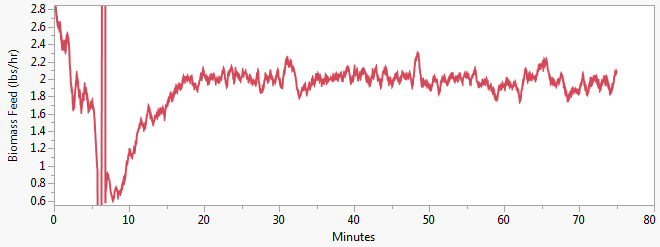
\includegraphics[width = \textwidth]{bm_good.png}
    \caption{Example of a biomass feed rate for a good experiment.  While biomass feed was unstable at the start of the run due to a bridge in the feeder, the feed rate recovered and was steady through a majority of the rest of the run.  A period from about 20 minutes to 55 minutes exists where feed rate oscilates by less than about $\pm$ 0.2 lbs/hr. }
    \label{bm_good}
\end{figure}

\begin{figure}[H]
    \centering
    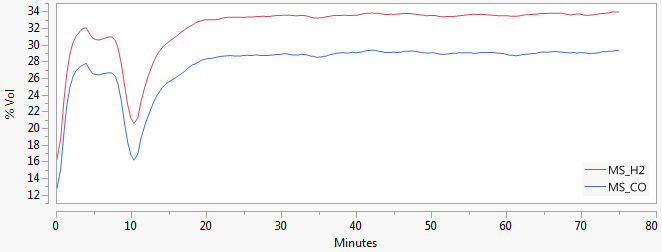
\includegraphics[width = \textwidth]{gas_good.png}
    \caption{Mass spec signals for carbon monoxide and hydrogen during a good experiment.  Because of the feed instability at the start of the run, the gas fractions are also inconsistent until the feed rate recovers and stabilizes.  However, a period from about 25 minutes into the run until the end exists where the volume fractions of carbon monoxide and hydrogen fluctuate by less than $\pm$ 0.5\% absolute.}
    \label{gas_good}
\end{figure}

\subsection*{Example of a Poor Run}

Relevant process data for another run which was completed recently is shown in Figures \ref{bm_bad}, \ref{gas_bad}, and \ref{temp_bad}.  This run is an example of a poor run in which no stady state existed.  There is no portion of this run which would qualify as either ``Good" or even ``Moderate" for analysis, and the best course of action for a run like this would be to end the experiment, evaluate what is causing the instabilities, rectify the problem, and re-try the run until it can be completed with a good steady state.

\begin{figure}[H]
    \centering
    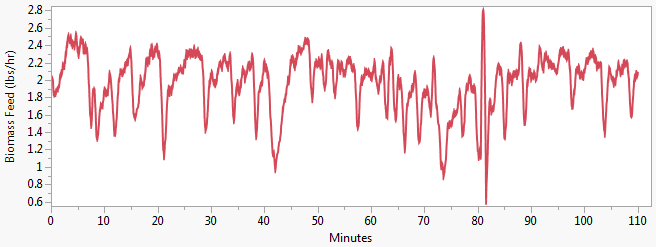
\includegraphics[width = \textwidth]{bm_bad.png}
    \caption{Biomass feed rates for a poor gasification experiment.  In spite of the length of this run being almost two hours, the feed rate fluctuates wildly throughout.  A portion of the run where biomass feed rate is steady at the set point does not exist.  This makes it impossible to choose a good block of time to analyze steady state behavior for the experiment.}
    \label{bm_bad}
\end{figure}

\begin{figure}[H]
    \centering
    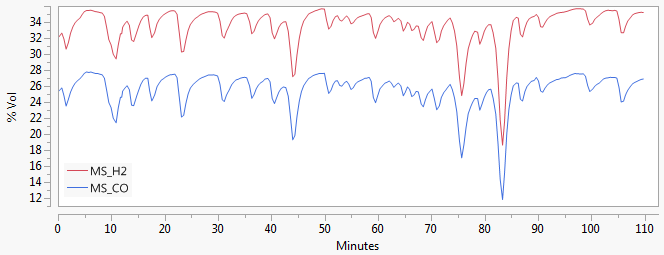
\includegraphics[width = \textwidth]{gas_bad.png}
    \caption{Because of the very unsteady biomass feed rate, gas species fractions from the mass spec are also unsteady.  Reading from the mass spec for carbon monoxide and hydrogen fluctuate by as much as $\pm$ 3\%.}
    \label{gas_bad}
\end{figure}

\begin{figure}[H]
    \centering
    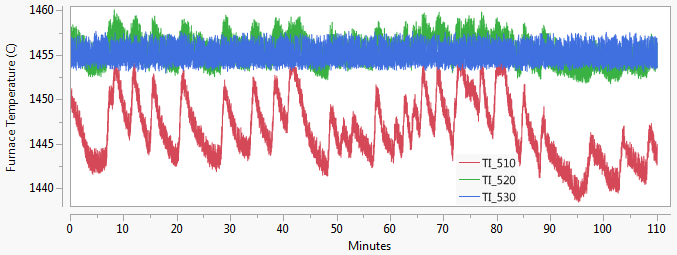
\includegraphics[width = \textwidth]{temp_bad.png}
    \caption{Biomass feed rate fluctuations also cause instability in the top zone of the SiC tube reactor.  This is another indication that there are problems in the system which are prohibiting steady state from being acheived.}
    \label{temp_bad}
\end{figure}


\section*{Conclusion}

It is important to consider the stability and accuracy of an experiment before it is finished and turned in as complete.  Also ensure before and during a run that setpoints for gas flows and reactor temperature are at the setpoint which is specified in the run plan.  When deciding if a run is satisfactorily complete for quality analyses, look for long term steady state periods during the run of at least 30 minutes.
\end{document}
